% -*- latex -*-
%%%%%%%%%%%%%%%%%%%%%%%%%%%%%%%%%%%%%%%%%%%%%%%%%%%%%%%%%%%%%%%%
%%%%%%%%%%%%%%%%%%%%%%%%%%%%%%%%%%%%%%%%%%%%%%%%%%%%%%%%%%%%%%%%
%%%%
%%%% This text file is part of the source of 
%%%% `Introduction to High-Performance Scientific Computing'
%%%% by Victor Eijkhout, copyright 2012-9
%%%%
%%%% This book is distributed under a Creative Commons Attribution 3.0
%%%% Unported (CC BY 3.0) license and made possible by funding from
%%%% The Saylor Foundation \url{http://www.saylor.org}.
%%%%
%%%%
%%%%%%%%%%%%%%%%%%%%%%%%%%%%%%%%%%%%%%%%%%%%%%%%%%%%%%%%%%%%%%%%
%%%%%%%%%%%%%%%%%%%%%%%%%%%%%%%%%%%%%%%%%%%%%%%%%%%%%%%%%%%%%%%%

\index{interoperability!C to Fortran|(}
\index{language interoperability|see{interoperability}}

Most of the time, a program is written is written in a single
language, but in some circumstances it is necessary or desirable to
mix sources in more than one language for a single executable. One
such case is when a library is written in one language, but used by a
program in another. In such a case, the library writer will probably
have made it easy for you to use the library; this section is for the
case that you find yourself in the place of the library writer. We
will focus on the common case of \emph{interoperability} between C/C++ and
Fortran.

This issue is complicated by the fact that both languages have
been around for a long time, and various recent language standards
have introduced mechanisms to facilitate interoperability.
However, there is still a lot of old code around, and not all compilers
support the latest standards. Therefore, we discuss both the old 
and the new solutions.

\Level 0 {Linker conventions}

As explained above, a compiler turns a source file into a binary,
which no longer has any trace of the source language: it contains in
effect functions in machine language. The linker will then match up
calls and definitions, which can be in different files. The problem
with using multiple languages is then that compilers have different
notions of how to translate function names from the source file to the
binary file.

Let's look at codes (you can find example files in \n{tutorials/linking}):
\begin{verbatim}
// C:
      Subroutine foo()
      Return
      End Subroutine
! Fortran
void foo() {
  return;
}
\end{verbatim}
After compilation you can use 
\indexterm{nm} to investigate the binary \indexterm{object file}:
\begin{verbatim}
%% nm fprog.o
0000000000000000 T _foo_
....
%% nm cprog.o
0000000000000000 T _foo
....
\end{verbatim}
You see that internally the \n{foo} routine has different names:
the Fortran name has an underscore appended. This makes
it hard to call a Fortran routine from~C, or vice versa.
The possible name mismatches are:
\begin{itemize}
\item The Fortran compiler appends an underscore. This is the most common case.
\item Sometimes it can append two underscores.
\item Typically the routine name is lowercase in the object file, but uppercase
      is a possibility too.
\end{itemize}

Since C is a popular language to write libraries in, this means
that the problem is often solved in the C library by:
\begin{itemize}
\item Appending an underscore to all C function names; or
\item Including a simple wrapper call:
\begin{verbatim}
int SomeCFunction(int i,float f)
{
  .....
}
int SomeCFunction_(int i,float f)
{
  return SomeCFunction(i,f);
}
\end{verbatim}
\end{itemize}

\Level 1 {C bindings in Fortran 2003}
 
With the latest Fortran standard there are explicit
\emph{C bindings}\index{Fortran!iso C bindings},
making
it possible to declare the
external name of variables and routines:
\verbatiminput{tutorials/linking/fbind.F90}
\begin{verbatim}
%% ifort -c fbind.F90
%% nm fbind.o
.... T _s
.... C _x
\end{verbatim}

It is also possible to declare data types to be C-compatible:
\verbatiminput{tutorials/linking/fdata.F90}

\Level 1 {C++ linking}
\index{C++!linking to|(}

Libraries written in C++ offer further problems.
The C++ compiler makes external symbols by combining
the names a class and its methods, in a process known
as \emph{name mangling}\index{C++!name mangling}.
You can force the compiler to
generate names that are intelligible to other languages by
\begin{verbatim}
#ifdef __cplusplus
  extern"C" {
#endif
  .
  .
  place declarations here
  .
  .
#ifdef __cplusplus
  }
#endif
\end{verbatim}

Example:
compiling
\begin{verbatim}
#include <stdlib.h>

int foo(int x) {
  return x;
}
\end{verbatim}
and inspecting the output with \n{nm} gives:
\begin{verbatim}
0000000000000010 s EH_frame1
0000000000000000 T _foo
\end{verbatim}
On the other hand, the identical program compiled as C++ gives
\begin{verbatim}
0000000000000010 s EH_frame1
0000000000000000 T __Z3fooi
\end{verbatim}
You see that the name for \n{foo} is something mangled, so you can not call 
this routine from a program in a different language. On the other hand,
if you add the \n{extern} declaration:
\begin{verbatim}
#include <stdlib.h>

#ifdef __cplusplus
  extern"C" {
#endif
int foo(int x) {
  return x;
}
#ifdef __cplusplus
  }
#endif
\end{verbatim}
you again get the same linker symbols as for~C, so that the routine
can be called from both C and~Fortran.

If your main program is in~C, you can use the C++ compiler as linker.
If the main program is in Fortran, you need to use the Fortran
compiler as linker. It is then necessary to link in extra
libraries for the C++ system routines. For instance, with the 
Intel compiler \n{-lstdc++ -lc} needs to be added to the link line.

The use of \n{extern} is also needed if you link other languages to a
C++ main program. For instance, a Fortran subprogram \n{foo} should be
declared as
\begin{verbatim}
extern "C" {
void foo_();
}
\end{verbatim}
In that case, you again use the C++ compiler as linker.

\index{C++!linking to|)}

\Level 1 {Complex numbers}

The \emph{complex data types in C/C++ and Fortran}%
\index{complex numbers!C and Fortran} are compatible with each
other. Here is an example of a C++ program linking to Lapack's complex
vector scaling routine~\indextermtt{zscal}.
%
\verbatimsnippet{zscale}

\Level 0 {Arrays}
\label{sec:CFarrays}
\index{C!array layout|(}
\index{Fortran!array layout|(}

C and Fortran have different conventions for storing multi-dimensional
arrays. You need to be aware of this when you pass an array between
routines written in different languages. 

Fortran stores multi-dimensional arrays in \indexterm{column-major}
order; see figure~\ref{fig:cf-arrays}.
For two dimensional arrays \texttt{A(i,j)} this means that
the elements in each column are stored contiguously: a $2\times2$
array is stored as \texttt{A(1,1), A(2,1), A(1,2), A(2,2)}. Three and
\begin{figure}[ht]
  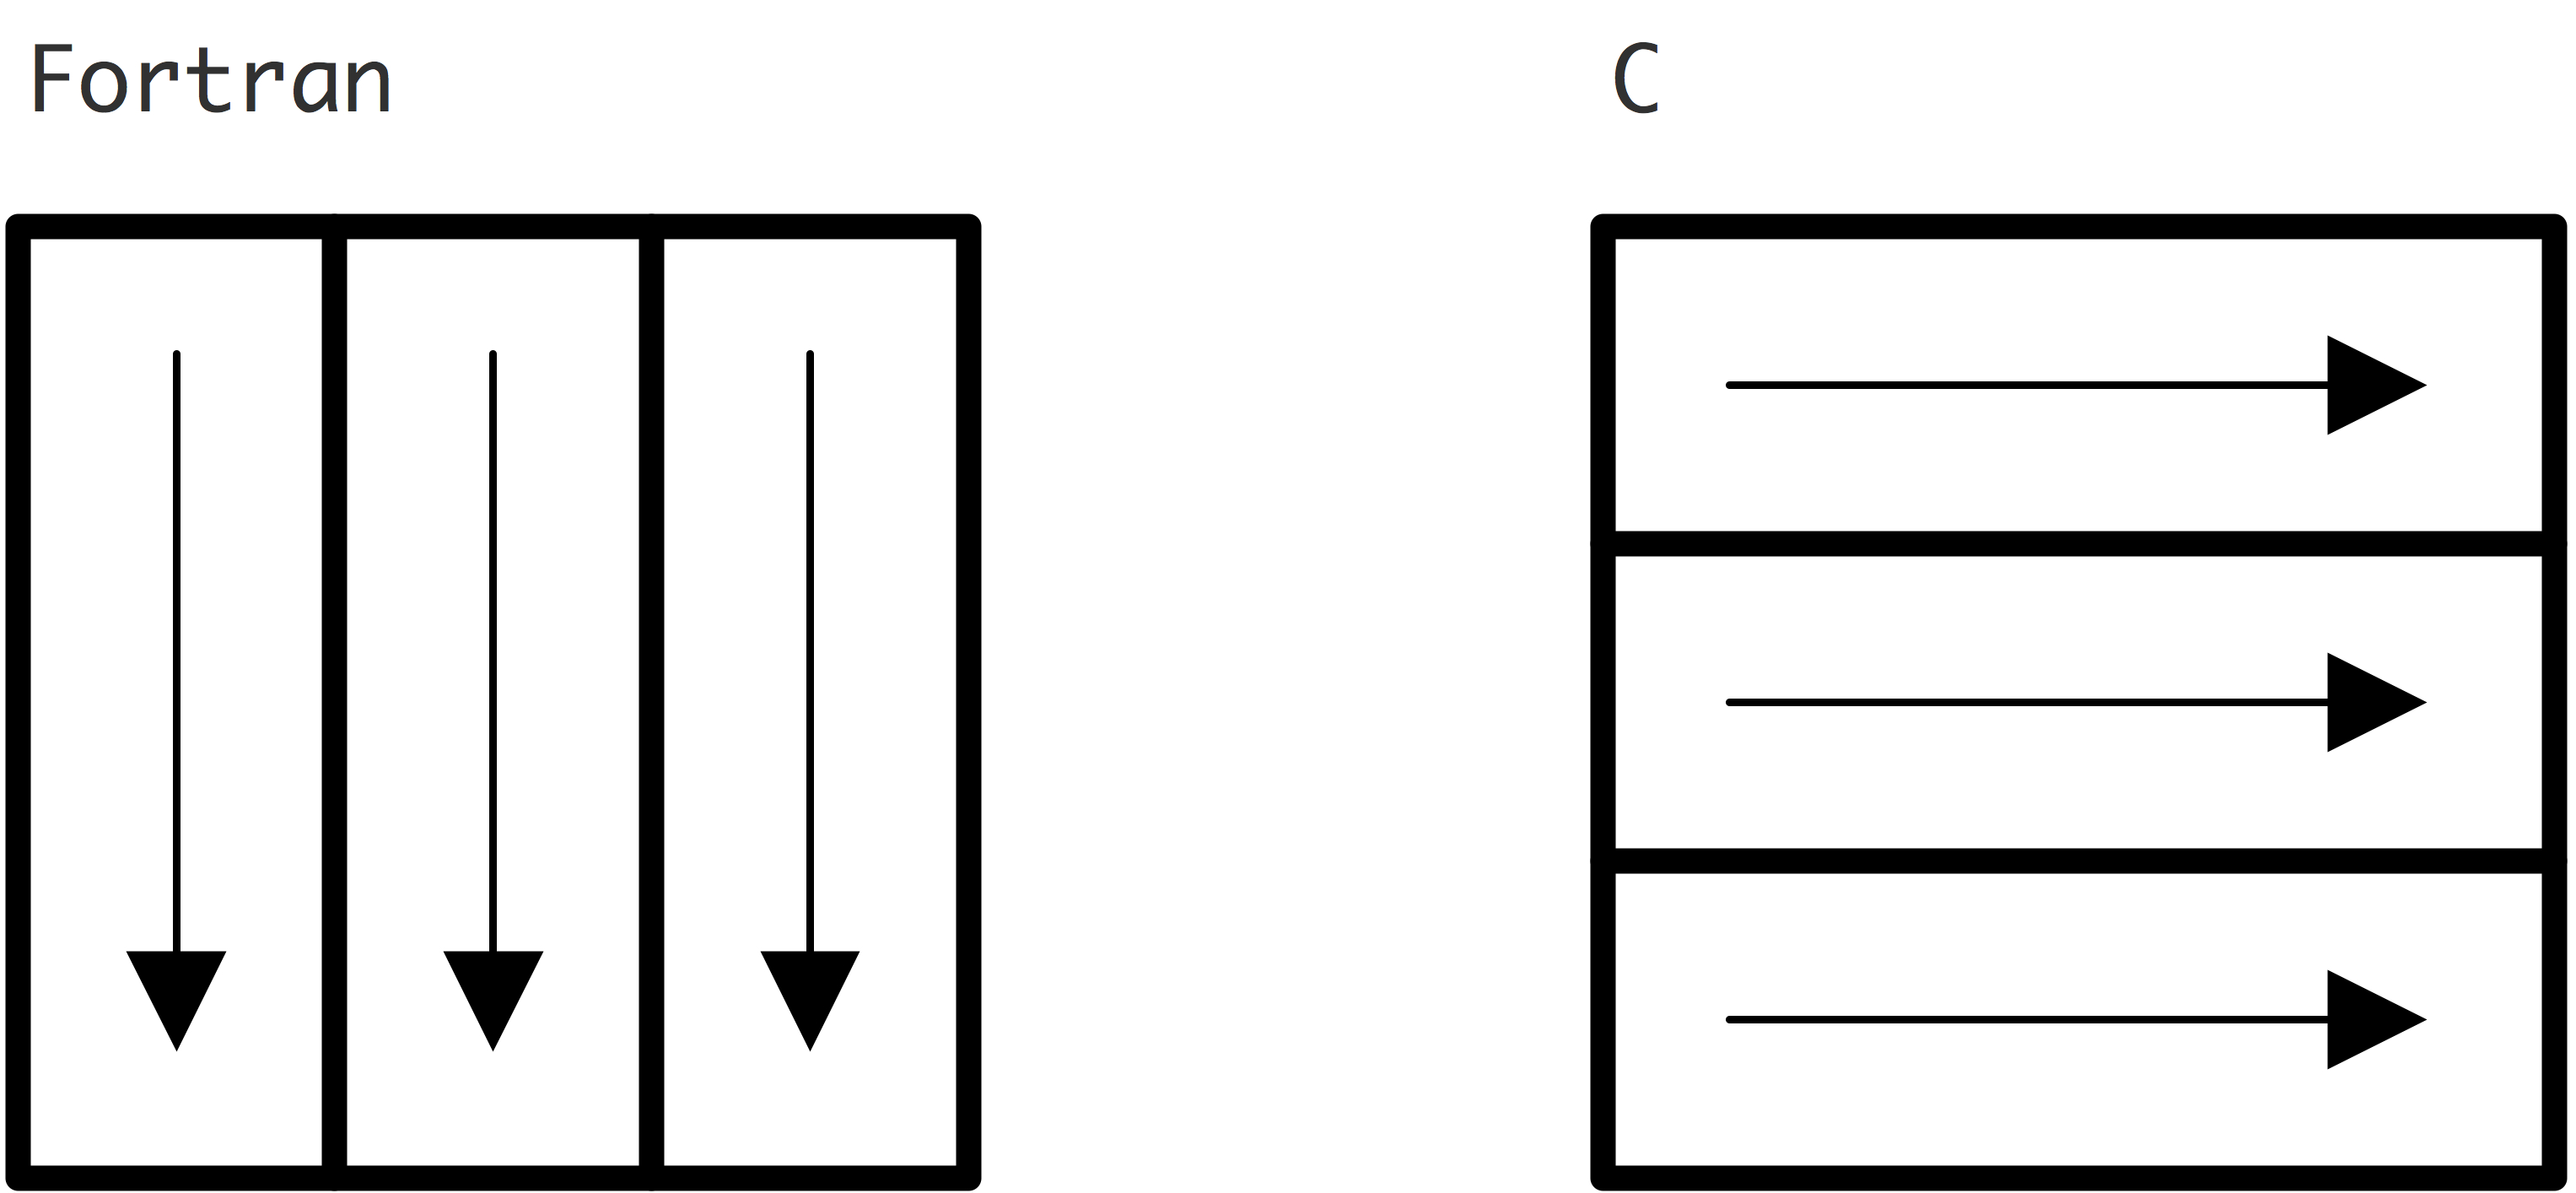
\includegraphics[scale=.13]{cf-arrays}
  \caption{Fortran and C array storage by columns and rows respectively}
  \label{fig:cf-arrays}
\end{figure}
higher dimensional arrays are an obvious extension: it is sometimes
said that `the left index varies quickest'.

C arrays are stored in \indexterm{row-major} order: elements in each
row are stored contiguous, and columns are then placed sequentially in
memory. A~$2\times2$ array \texttt{A[2][2]} is stored as
\texttt{A[1][1], A[1][2], A[2][1], A[2][2]}. 

A number of remarks about arrays in~C.
\begin{itemize}
\item C (before the C99 standard) has multi-dimensional arrays only in
  a limited sense. You can declare them, but if you pass them to another
  C function, they no longer look multi-dimensional: they have become
  plain \texttt{float*} (or whatever type) arrays. That brings us to
  the next point.
\item Multi-dimensional arrays in C look as if they have type
  \texttt{float**}, that is, an array of pointers that point to
  (separately allocated) arrays for the rows. While you could
  certainly implement this:
\begin{verbatim}
float **A;
A = (float**)malloc(m*sizeof(float*));
for (i=0; i<n; i++)
  A[i] = (float*)malloc(n*sizeof(float));
\end{verbatim}
  careful reading of the standard reveals that a multi-dimensional
  array is in fact a single block of memory, no further pointers
  involved.
\end{itemize}
Given the above limitation on passing multi-dimensional arrays, and
the fact that a C~routine can not tell whether it's called from
Fortran or~C, it is best not to bother with multi-dimensional arrays
in C, and to emulate them:
\begin{verbatim}
float *A;
A = (float*)malloc(m*n*sizeof(float));
#define SUB(i,j,m,n) i+j*m
for (i=0; i<m; i++)
  for (j=0; j<n; j++)
    .... A[SUB(i,j,m,n)] ....
\end{verbatim}
where for interoperability we store the elements in column-major fashion.

\index{C!array layout|)}
\index{Fortran!array layout|)}

\Level 1 {Array alignment}
\index{cacheline!boundary alignent|seealso{allocation, aligned}}

For reasons such as \ac{SIMD} \indexterm{vector instructions}, it can
be advantageous to use \indextermsubdef{aligned}{allocation}. For
instance, `16-byte alignment' means that the starting address of your
array, expressed in bytes, is a multiple of~16.

In~C, you can force such alignment with 
\indextermtt{posix\_memalign}. In Fortran there is no general
mechanism for this. The Intel compiler allows you to write:
\begin{verbatim}
double precision, allocatable :: A(:), B(:)
!DIR$ ATTRIBUTES ALIGN : 32 :: A, B
\end{verbatim}

\Level 0 {Strings}

Programming languages differ widely in how they handle strings. 
\begin{itemize}
\item In C, a string is an array of characters; the end of the string
  is indicated by a null character, that is the ascii character zero,
  which has an all zero bit pattern. This is called \indexterm{null
    termination}.
\item In Fortran, a string is an array of characters. The length is
  maintained in a internal variable, which is passed as a hidden
  parameter to subroutines.
\item In Pascal, a string is an array with an integer denoting the
  length in the first position. Since only one byte is used for this,
  strings can not be longer than 255 characters in Pascal.
\end{itemize}
As you can see, passing strings between different languages is fraught
with peril. This situation is made even worse by the fact that passing
strings as subroutine arguments is not standard.

Example: the main program in Fortran passes a string
\verbatiminput{tutorials/linking/fstring.F90}
and the C routine accepts a character string and its length:
\verbatiminput{tutorials/linking/cstring.c}
which produces:
\begin{verbatim}
length = 5
<<Word >>
\end{verbatim}

To pass a Fortran string to a C program you need to append a null
character:
\begin{verbatim}
call cfunction ('A string'//CHAR(0))
\end{verbatim}
Some compilers support extensions
to facilitate this, for instance writing
\begin{verbatim}
DATA forstring /'This is a null-terminated string.'C/
\end{verbatim}
Recently, the `C/Fortran interoperability standard' has
provided a systematic solution to this.

\Level 0 {Subprogram arguments}

In C, you pass a \texttt{float} argument to a function if the function
needs its value, and \texttt{float*} if the function has to modify the
value of the variable in the calling environment. Fortran has no such
distinction: every variable is passed \indexterm{by reference}. This
has some strange consequences: if you pass a literal value
\texttt{37} to a subroutine, the compiler will allocate a nameless
variable with that value, and pass the address of it, rather than the
value\footnote{With a bit of cleverness and the right compiler, you
  can have a program that says \texttt{print *,7} and
  prints~\texttt{8} because of this.}.

For interfacing Fortran and C routines, this means that a Fortran
routine looks to a C~program like all its argument are `star'
arguments. Conversely, if you want a C subprogram to be callable from
Fortran, all its arguments have to be star-this or that. This means on
the one hand that you will sometimes pass a variable by reference that
you would like to pass by value.

Worse, it means that C subprograms like
\begin{verbatim}
void mysub(int **iarray) {
 *iarray = (int*)malloc(8*sizeof(int));
 return;
}
\end{verbatim}
can not be called from Fortran. There is a hack to get around this
(check out the Fortran77 interface to the Petsc routine
\texttt{VecGetValues}) and with more cleverness you can use
\texttt{POINTER} variables for this.

\Level 0 {Input/output}

Both languages have their own system for handling input/output, and it
is not really possible to meet in the middle. Basically, if Fortran
routines do I/O, the main program has to be in Fortran. Consequently,
it is best to isolate I/O as much as possible, and use C for I/O in
mixed language programming.

\Level 0 {Fortran/C interoperability in Fortran2003}

The latest version of Fortran, unsupported by many compilers at this
time, has mechanisms for interfacing to~C.
\begin{itemize}
\item There is a module that contains named kinds, so that one can declare
\begin{verbatim}
INTEGER,KIND(C_SHORT) :: i
\end{verbatim}
\item Fortran pointers are more complicated objects, so passing them
  to~C is hard; Fortran2003 has a mechanism to deal with C~pointers,
  which are just addresses.
\item Fortran derived types can be made compatible with C~structures.
\end{itemize}

\index{interoperability!C to Fortran|)}

\Level 0 {Python calling C code}

\index{interoperability!C to python|(}

Because of its efficiency of computing, C~is a logical language to use
for the lowest layers of a program. On the other hand, because of its
expressiveness, Python is a good candidate for the top layers. It is
then a logical thought to want to call C~routines from a python
program.
%
This is possible using the python \emph{ctypes}\index{ctypes (python module)}
module.
\begin{enumerate}
\item You write your C code, and compile it to a dynamic library as
  indicated above;
\item The python code loads the library dynamically, for instance for
  \indextermtt{libc}:
\begin{verbatim}
path_libc = ctypes.util.find_library("c")
libc = ctypes.CDLL(path_libc)
libc.printf(b"%s\n", b"Using the C printf function from Python ... ")
\end{verbatim}
\item You need to declare what the types are of the C routines in python:
\begin{verbatim}
test_add = mylib.test_add
test_add.argtypes = [ctypes.c_float, ctypes.c_float]
test_add.restype = ctypes.c_float
test_passing_array = mylib.test_passing_array
test_passing_array.argtypes = [ctypes.POINTER(ctypes.c_int), ctypes.c_int]
test_passing_array.restype = None
\end{verbatim}
\item Scalars can be passed simply; arrays need to be constructed:
\begin{verbatim}
data = (ctypes.c_int * Nelements)(*[x for x in range(numel)])
\end{verbatim}
\end{enumerate}

\index{interoperability!C to python|)}
